
%
% a front end for the draft
%
% This version is actually what I gave to my committee
% and published as a tech report.
% IMHO, the report style is much better for human consumption
% than the required thesis style.
%    -johnh, 12-Jan-96
%

\newif\ifissubmit
\issubmitfalse

\newif\ifisdraft
\isdrafttrue

% \documentclass[PhD,single,twoside]{uclathes}
\documentclass[twocolumn,twoside]{book}
\usepackage{times}

%%%%%%%%%%%%%%%%%%%%%%%%%%%%%%%%%%%%%%%%%%%%%%%%%%%%%%%%%%%%%%%%%%%%%%
%
% format hacking:
%

\makeatletter

  %
  % get the thesis title page format
  %
  \input{uclathma.clo}
  \input{uclathti.clo}

  %
  % sectiion titles
  %
  \renewcommand\section{\@startsection {section}{1}{\z@}%
                                     {-3.5ex \@plus -1ex \@minus -.2ex}%
                                     {2.3ex \@plus.2ex}%
                                     {\reset@font\Large\bfseries\nohyphenation}}
  \renewcommand\subsection{\@startsection{subsection}{2}{\z@}%
                                       {-3.25ex\@plus -1ex \@minus -.2ex}%
                                       {1.5ex \@plus .2ex}%
                                       {\reset@font\large\bfseries\nohyphenation}}
  \renewcommand\subsubsection{\@startsection{subsubsection}{3}{\z@}%
                                       {-3.25ex\@plus -1ex \@minus -.2ex}%
                                       {1.5ex \@plus .2ex}%
                                       {\reset@font\normalsize\bfseries\nohyphenation}}
  \renewcommand\paragraph{\@startsection{paragraph}{4}{\z@}%
                                      {3.25ex \@plus1ex \@minus.2ex}%
                                      {-1em}%
                                      {\reset@font\normalsize\bfseries\nohyphenation}}
  \renewcommand\subparagraph{\@startsection{subparagraph}{5}{\parindent}%
                                         {3.25ex \@plus1ex \@minus .2ex}%
                                         {-1em}%
                                        {\reset@font\normalsize\bfseries\nohyphenation}}

  %
  % Steal the bibliography from uclathes so it's a real chapter.
  %
  \def\thebibliography#1{\chapter*{References\markboth
    {REFERENCES}{REFERENCES}}
    \addcontentsline{toc}{chapter}{References}
    \renewcommand\baselinestretch{1}
    \@normalsize
    \list{[\arabic{enumi}]}{\settowidth\labelwidth{[#1]}\leftmargin\labelwidth
      \advance\leftmargin\labelsep
      \usecounter{enumi}}
      \def\newblock{\hskip .11em plus .33em minus -.07em}
      \sloppy
      \sfcode`\.=1000\relax}
  
  \def\endthebibliography{\renewcommand\baselinestretch{\@spacing}\@normalsize\endlist}
  
  %
  % margin hacking
  %
  %
  % First get rid of driver margins.
  \setlength{\voffset}{-1in}
  \setlength{\hoffset}{-1in}
  % Set column width and gutter
  \setlength{\textheight}{8.5in}
  % Top and bottom margins.
  \setlength{\topmargin}{0.75in}
  \setlength{\headheight}{12\p@}
  \setlength{\headsep}{0.25in}
  \setlength{\footskip}{0.35in}
  % Left and right margins.
  \setlength{\evensidemargin}{0.80in}
  \setlength{\oddsidemargin}{1.25in}
  % width
  \setlength{\textwidth}{6.45in}
  \setlength{\columnsep}{0.25in}


\makeatother



%
% main.tex
% Copyright (C) 1995 by John Heidemann, <johnh@isi.edu>.
% $Id: demo2big.tex,v 1.2 1996/01/16 18:57:04 johnh Exp $
%


%
% thesis_macros
% Copyright (C) 1995 by John Heidemann, <johnh@isi.edu>
%

% \RequirePackage{johnh_general}

\RequirePackage{ifthen}

% \def\epsfreduction{0.667}
\def\epsfgraphreduction{0.9}

\newcommand\comment[1]{{[\sffamily #1]}}

%
% TeX seems to want to indent after chapters,
% although it shouldn't.  Rather than argue
% with it, I work around it manually by putting this
% hack in the right places:
\newcommand{\noindenthack}{\noindent}


\newcommand{\fwling}{featherweight layering}
\newcommand{\fwls}{featherweight layers}
\newcommand{\fwl}{featherweight layer}

\newcommand{\Fwling}{Featherweight layering}
\newcommand{\Fwls}{Featherweight layers}
\newcommand{\Fwl}{Featherweight layer}

\newcommand{\FwLing}{Featherweight Layering}
\newcommand{\FwLs}{Featherweight Layers}
\newcommand{\FwL}{Featherweight Layer}

\newcommand{\xvop}[2]{{\scomputer {{#1}\_{#2}}}}
\newcommand{\vop}[1]{\xvop{vop}{#1}}

\newcommand{\usec}{$\mu$seconds}
\newcommand{\unix}{Unix}

\newcommand{\dotdot}{\scomputer{..}}

\newenvironment{mycode}%
	{\small
	}{%
	}

\newcommand{\mylangle}{\langle}
\newcommand{\myrangle}{\rangle}
\newcommand{\myrightarrow}{\rightarrow}


%
% Sizes of various things:
%
  \newcommand{\tablesize}{\normalsize}
  \newcommand{\computertablesize}{\small}
  \newcommand{\bibliographysize}{\normalsize}

  %
  % Another space-saver:  shrink the figures and graphs.
  %
 \def\epsfreduction{0.85}
 \def\epsfgraphreduction{0.9}   % should be left at 0.9 with two-column text
% \def\epsfsize#1#2{\epsfreduction#1}

%\newcommand{\appendixnumbering}{
%	\renewcommand{\thechapter}{\Alph{chapter}}
%	\setcounter{chapter}{0}
%	}

\newenvironment{functions}%
	{\begin{description}}%
	{\end{description}}

\makeatletter
  \newcommand{\SubmitSingleSpace}{
    \ifissubmit
      \renewcommand\baselinestretch{\@singlespacing}\@normalsize
    \fi
  }
  \newcommand{\SubmitDoubleSpace}{
    \ifissubmit
      \renewcommand\baselinestretch{\@doublespacing}\@normalsize
    \fi
  }
\makeatother


\iffalse
Figure drawing style guide:

layer labels:
	helvetica 12pt bold
	(short acronyms) helvetica 14pt bold

spacing:  8 pixels
each layers will be 3 high and 7 or 7.5 wide

or spacing: 8 pts
each layer will be 4 high and 10 wide

boxes and vnode links are line #2
\fi



\begin{document}


%
% Title pages of the thing
% Copyright (C) 1995 by John Heidemann, <johnh@isi.edu>.
%



\title{\textbf{Stackable Design of File Systems}}
\author{John~Shelby Heidemann}


\department{Computer Science}
\degreemonth{September}
\degreeyear{1995}

\chair{Gerald~J.~Popek}
\chair{D.~Stott Parker}
\member{Richard~Muntz}
\member{Rajive~L.~Bagrodia}
\member{Kirby~A.~Baker}

\dedication{\textsl{Are you dedicated?}}

\acknowledgments{
Ack!  P'tui.
}

%%%%%%%%%%%%%%%%%%%%%%%%%%%%%%%%%%%%%%%%%%%%%%%%%%%%%%%%%%%%%%%%%%%%%%
%
% vita
%
\vitaitem{1968}{Born, Syracuse, New York, USA.}
\vitaitem{etc.}{etc.}
\vitaitem{1995}{Graduated, UCLA}

%%%%%%%%%%%%%%%%%%%%%%%%%%%%%%%%%%%%%%%%%%%%%%%%%%%%%%%%%%%%%%%%%%%%%%
%
% publications
%

\publication{
	Richard~G.\ Guy, John~S.\ Heidemann, Wai Mak, Thomas~W.\ Page,~Jr.,\ 
	  Gerald~J.\ Popek, and Dieter Rothmeier.
	Implementation of the Ficus
	  replicated file system.
	In \emph{USENIX Conference Proceedings}, pages
	  63--71.
	USENIX, June 1990.
}

\publication{
	etc.
}




%%%%%%%%%%%%%%%%%%%%%%%%%%%%%%%%%%%%%%%%%%%%%%%%%%%%%%%%%%%%%%%%%%%%%%


% Abstract
\clearpage
\thispagestyle{plain}
\phantomsection
\addcontentsline{toc}{chapter}{Abstract}

\centerline{\zihao{3}\bfseries Abstract}

\linespread{1.4}\zihao{-4}
\bigskip

This thesis explores the relationship between focus structure and pronoun resolution among non-native speakers of English and French. Firstly we reviewed the existing literature on the mechanism of focus effect and pronoun resolution. Then through a self-paced reading test, we find that focus, in the form of cleft structure does not necessarily increase the salience of a informational unit, thus may not in some cases make it a preferred antecedent for pronoun resolution. This result is line with previous researches on this topic. In our experiment, We also find that focused subject in French and focused object in English are processed faster, but focused subjects in both languages leads to longer response time of anaphora. Furthermore, our research also shows that the congruence between anaphora and focus does not make the latter more accessible. In this regard, we argue that the problem of whether there is subject or object preference in English and French is more complicated than the results of current studies.

\bigskip
\noindent\textbf{\zihao{4} Keywords:} 
focus effect, pronoun resolution, self-paced reading, English, French



%
% I built a custom title page to do what I want.  So sue me.
% NEEDSWORK:  I had to copy some stuff from uclathti.sty.
%
\makeatletter
  \newcommand{\CustomTitlePage}{
    \begin{titlepage}
      \ColumnSave
      \vspace*{1.5in}   % a hacky way to center.  TeX didn't like \vfill.
      \begin{center}
  
      {\bfseries\huge \@title} \\
      \vskip 48pt plus0pt minus18pt
  
      {\large \@author} \\
      \vskip 12pt plus0pt minus3pt
      {\large University of California, Los Angeles} \\
      \vskip 6pt plus0pt minus2pt
      {\large \@degreemonth, \@degreeyear} \\
      \vskip 48pt plus0pt minus18pt
  
      \normalsize A \@thesisname\
      submitted in partial satisfaction \\
      of the requirements for the degree \\
      \@degreename\if@department\ in \@department \fi\\
      \vskip 24pt plus0pt minus6pt

      \normalsize
	UCLA Computer Science Department \\
	Technical Report UCLA-CSD-950032 \\
      \vskip 24pt plus0pt minus6pt

      \textbf{Thesis committee:} \\
      \ifnum\c@chairs<1
        \typeout{No committee chair.}
      \else\ifnum\c@chairs<2
        \@chairA, chair \\
      \else\ifnum\c@chairs<3
        \@chairA, co-chair \\
        \@chairB, co-chair \\
      \else\ifnum\c@chairs<4
        \@chairA, co-chair \\
        \@chairB, co-chair \\
        \@chairC, co-chair \\
      \fi\fi\fi\fi
      \ifnum\c@members<1 \typeout{No non-chair committee members.}\fi
      \ifnum\c@members>0 \@memberA \\ \fi
      \ifnum\c@members>1 \@memberB \\ \fi
      \ifnum\c@members>2 \@memberC \\ \fi
      \ifnum\c@members>3 \@memberD \\ \fi
      \ifnum\c@members>4 \@memberE \\ \fi
      \ifnum\c@members>5 \@memberF \\ \fi

      \end{center}
    \end{titlepage}
  }

  \newcommand{\CustomAcknowledgePage}{
  \chapter*{Acknowledgments}

  \@acknowledgments
  }
\makeatother

\ifissubmit
  \makeintropages
\else
  \makeatletter
    \pagenumbering{roman}
    \CustomTitlePage
    \@makecopyrightpage
    \@makededication
    \tableofcontents
    \listoffigures
    \listoftables
    \cleardoublepage
    \@makeabstractpage{1.0}
    \CustomAcknowledgePage
%    \@makevitapage

    \cleardoublepage
    \pagestyle{headings}
    \pagenumbering{arabic}
    \setcounter{page}{1}
  \makeatother
\fi


% LocalWords:  Stott Muntz Ted Yu Wu Michial Gunter Stovall Salomone Louie Qian
% LocalWords:  Qin Weidner McKusick Pendry Minshall kitrace Ousterhout CSD ftp
% LocalWords:  Administrativia csd ps HyperCard Yarvis Alexy Rudenko pt Los co
% LocalWords:  degreemonth degreeyear thesisname degreename chairA chairB roman
% LocalWords:  chairC memberA memberB memberC memberD memberE memberF arabic
% LocalWords:  makecopyrightpage makededication makeabstractpage Monique http
% LocalWords:  Bennarosh www html


%
% introduction.tex
% Copyright (C) 1995 by John Heidemann, <johnh@isi.edu>.
% $Id: demo2int.tex,v 1.1 1996/01/12 18:13:58 johnh Exp $
%

\chapter{Introduction}

\noindenthack
Filing services are one of the most user-visible
  parts of the operating system,
  so it is not surprising that 
  many new services are proposed
  by researchers
  and that a variety of third parties are interested in providing
  these solutions.
Of the many innovations which have been proposed,
  very few have become widely available
  in a timely fashion.
We believe this delay results from two deficiencies
  in practices of current file-system development.
First,
  file systems are large and difficult to implement.
This problem is compounded because
  no good mechanism exists to allow
  new services to build on those which already exist.
Second,
  file systems today are built around a few fixed interfaces
  which fail to accommodate the change and evolution inherent in
  operating systems development.
Today's filing interfaces vary from
  system to system,
  and even between point releases of a 
  single operating system.
These differences greatly complicate and therefore discourage
  third-party development and adoption of filing extensions.

These problems raise barriers to the widespread
  development, deployment, and maintenance of new filing
  services.
The thesis of this dissertation is that
  a layered,
  \emph{stackable} structure
  with an \emph{extensible} interface
  provides a much better methodology
  for file-system development.
We propose construction of filing services from a number
  of potentially independently developed modules.
By stackable,
  we mean that these modules are bounded by
  identical, or \emph{symmetric}, interfaces above and below.
By extensible, we mean that these interfaces
  can be independently changed by multiple parties,
  without invalidating existing or future work.

To validate this thesis we developed a
  framework supporting stackable file-systems
  and used that framework to construct several
  different filing services.
This dissertation describes the design,
  implementation,
  and evaluation of this system.


% \input{motivation}



% \section{Related Work}
%	\label{sec:intro_related_work}

% ...


% LocalWords:  Posix Novell's Netware Kernighan Madnick Alsop NeFS PostScript
% LocalWords:  Rosenthal SunSoft NEEDSWORK Wong

%...
%\input{stacking_model}
%\input{stacking_techniques}
%\input{stacking_implementation}
%\input{stacking_evaluation}
%\input{coherence_architecture}
%\input{coherence_implementation}
%\input{coherence_evaluation}
%\input{fwl_implementation}
%\input{fwl_evaluation}
%\input{related_work}
%% !Mode:: "TeX:UTF-8" 
\begin{conclusions}

学位论文的结论作为论文正文的最后一章单独排写,但不加章标题序号。

结论应是作者在学位论文研究过程中所取得的创新性成果的概要总结,不能与摘要混为一谈。博士学位论文结论应包括论文的主要结果、创新点、展望三部分,在结论中应概括论文的核心观点,明确、客观地指出本研究内容的创新性成果(含新见解、新观点、方法创新、技术创新、理论创新),并指出今后进一步在本研究方向进行研究工作的展望与设想。对所取得的创新性成果应注意从定性和定量两方面给出科学、准确的评价,分(1)、(2)、(3)…条列出,宜用“提出了”、“建立了”等词叙述。

\end{conclusions}


%\appendix
%\input{stacking_appendix}
%\input{coherence_appendix}

%\bibliographystyle{uclathes}
%\bibliography{ficus,thesis}

%%!TEX root = ../dissertation.tex
\newpage

% If you do want an image in the colophon:
\begin{figure}
  \vspace{20pt}
  \centering
  \hspace*{-32pt}
  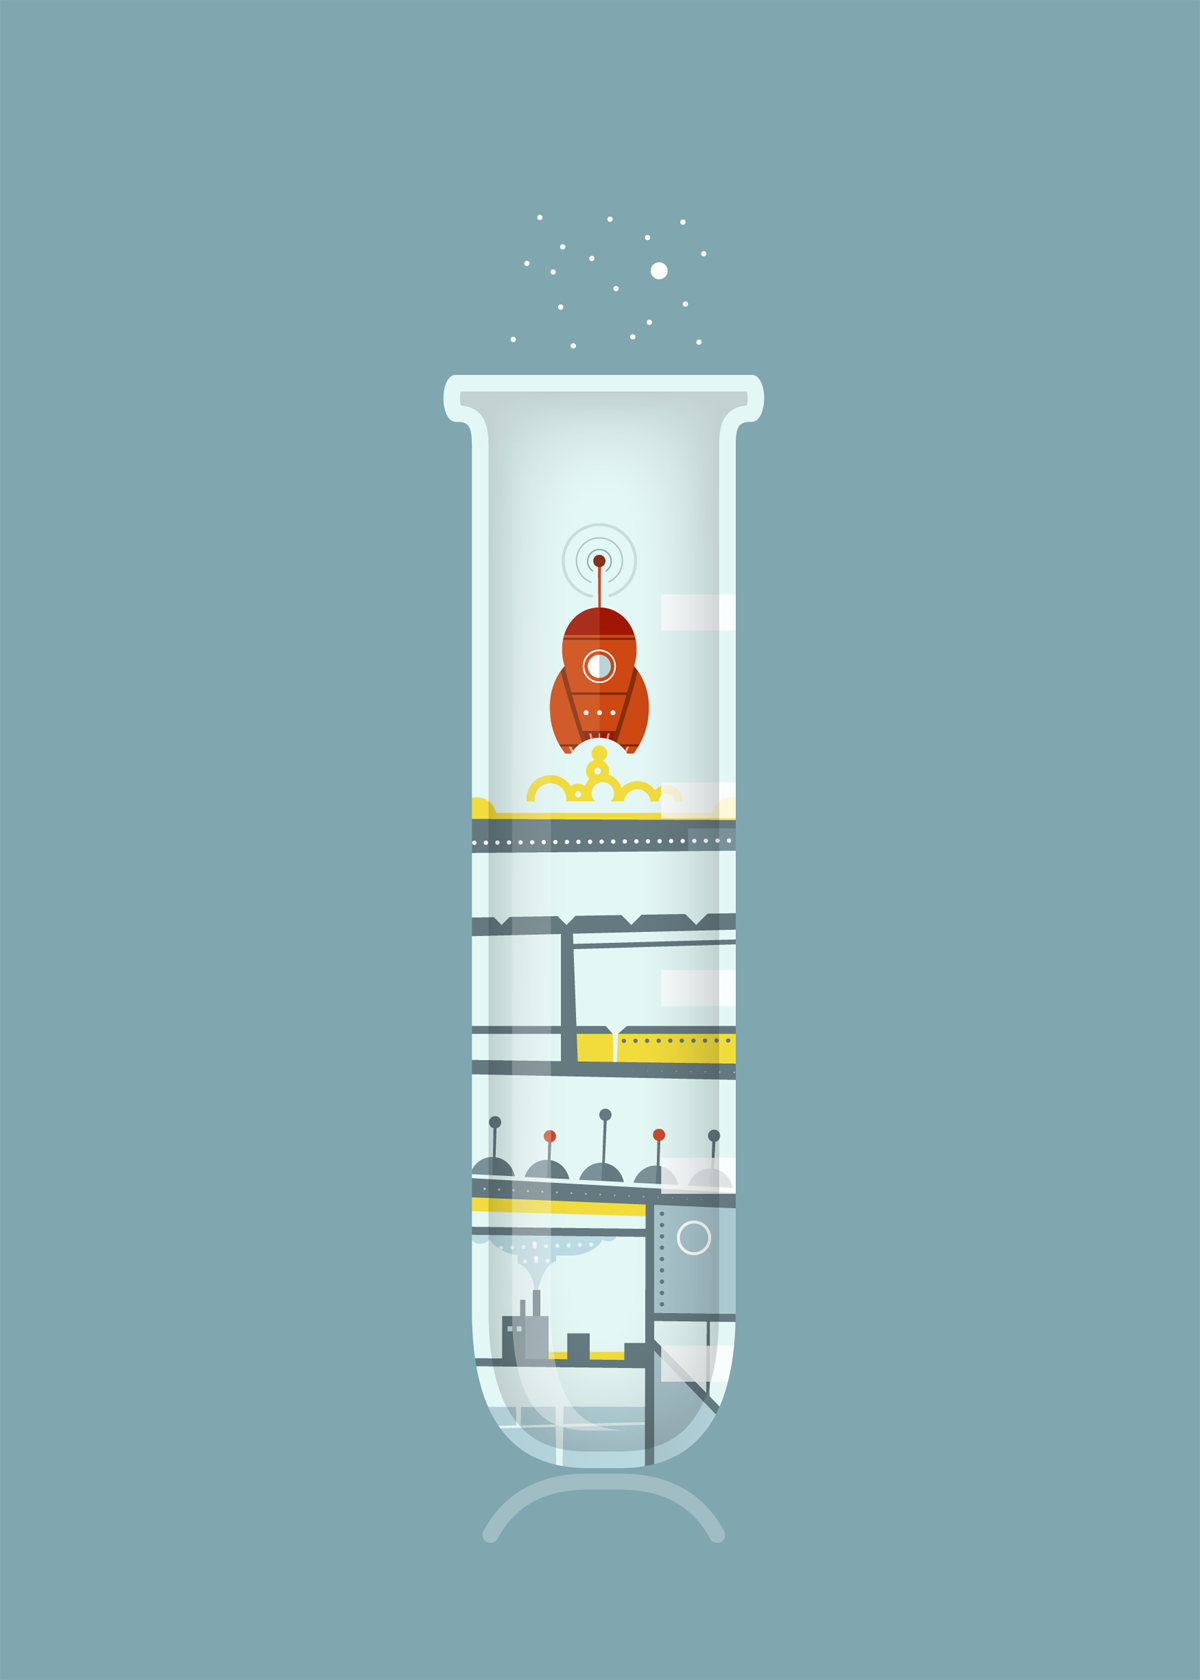
\includegraphics[width=0.42\textwidth]{endmatter/colophon.png}
\end{figure}

% If you don't want an image in the colophon:
% \vspace*{200pt}

\begin{center}
\parbox{200pt}{\lettrine[lines=3,slope=-2pt,nindent=-4pt]{\textcolor{SchoolColor}{T}}{his thesis was typeset} using \LaTeX, originally developed by Leslie Lamport and based on Donald Knuth's \TeX. The body text is set in 11 point Egenolff-Berner Garamond, a revival of Claude Garamont's humanist typeface. The above illustration, \textit{Science Experiment 02}, was created by Ben Schlitter and released under \href{http://creativecommons.org/licenses/by-nc-nd/3.0/}{\textsc{cc by-nc-nd 3.0}}. A template that can be used to format a PhD dissertation with this look \textit{\&} feel has been released under the permissive \textsc{agpl} license, and can be found online at \href{https://github.com/suchow/Dissertate}{github.com/suchow/Dissertate} or from its lead author, Jordan Suchow, at \href{mailto:suchow@post.harvard.edu}{suchow@post.harvard.edu}.}
\end{center}


\end{document}


